% Same-visit cosmic-ray check (banzai_floyds/visit_cosmics.py), input from ch11_cosmics.tex
\section{The second exposure of the visit}
\label{sec:cr_pair}
\textit{The problem.} With the object model, LA Cosmic searches the right residual, but it still has to judge a sharp
feature by its shape alone. A narrow line from a resolved narrow-line region can be as sharp as a cosmic ray (the 15
H$\alpha$ pixels of Fig.~\ref{fig:cr_method}). \textit{The idea.} The visits of the reverberation-mapping programme have
two exposures of the same pointing, taken back to back. A cosmic ray lands in only one of them; a line, a star core, a
sky line or a fringe is in both. The other exposure of the visit (the \textit{partner}) is therefore the most direct
test there is. \textit{The change.} We have added this test to the pipeline as a stage that runs right after LA Cosmic
and that we call the \textit{same-visit check} (code: \texttt{SameVisitCosmicRays} in
\texttt{banzai\_floyds/visit\_cosmics.py}). It removes the LA Cosmic flags on features that the partner also shows,
and adds strong, compact hits that LA Cosmic missed. \textit{Tests and result}
(Sections~\ref{sec:cr_pair_inject} and \ref{sec:cr_pair_sample}): it finds the same artificial cosmic rays as the
object model alone, flags 10--22 per cent fewer pixels, and clears the H$\alpha$ peak of
Fig.~\ref{fig:cr_halpha}.

For a frame $a$ with partner $b$, the check does the following.
\begin{enumerate}
\item \textit{Find the partner}: among the raw frames of the same night in the folder of the frame, those of the same
type and the same LCO \textit{molecule} (the group of exposures taken together within one request; header keyword
\texttt{MOLUID}), the nearest in time first. A frame without a partner keeps the LA Cosmic flags of
Section~\ref{sec:cr_model}. This is the case for all the standards, which are single exposures.
\item \textit{Reduce the partner} up to and including LA Cosmic, in the same way as the frame (no database records are
written for it). Each exposure is sky-subtracted with its own sky model.
\item \textit{Shift the partner along the slit} onto the trace of the frame. The shift is the difference of the fitted
trace centres in each column, smoothed over 15 columns. Where the object is bright (S/N of the column above 30), it is
refined by the difference of the flux centroids within 2\,FWHM of the trace, smoothed over 5 columns. This refinement
is needed because the trace centres follow the continuum, while the narrow-line region of NGC\,4151 can sit up to half a
pixel away, and a half-pixel offset turns the peak of a bright line into a positive--negative pattern in the difference
with the partner.
\item \textit{Scale the partner} in each column by the median ratio $a/b$ over the trace core, smoothed over 31
columns. Where the object is faint, the ratio of the exposure times is used.
\item \textit{Shift the partner along the dispersion.} In a wide slit, the position of the object across the slit
shifts its spectrum. The two exposures of a visit differ by 0.1\,pixel (median) at OGG and 0.3\,pixel at COJ, and by up
to 0.6 and 1.2\,pixels; this puts the flanks of a bright narrow line out of step. The offset is measured for each order
from the cross-correlation of the two spectra summed over the trace (a parabola through its peak). Where it exceeds
0.1\,pixel, it is removed by resampling the partner with a cubic spline. The offset is used only where the peak of the
normalised cross-correlation exceeds 0.5, because a spectrum with no features above the noise has no offset to measure
(Section~\ref{sec:cr_pair_sample}). It is recorded in the header keywords \texttt{L1CRDX1} and \texttt{L1CRDX2} (red
and blue order).
\item \textit{Match the partner to the frame.} The seeing changes within a visit. For example, the FWHM of Fairall\,9
went from 11.6 to 14.7\,pixels between the two exposures of 2026 September 6 (and its flux changed by a factor 0.63);
a scale and a shift cannot absorb that. As in image subtraction \citep{Alard1998}, the partner is therefore convolved
with a kernel along the slit, fitted to the frame:
\[
m(y)=\sum_{|k|\le6}c_k\,s\,b(y+k)+c_{\rm sky}+c'_{\rm sky}\,y ,
\]
where $m$ is the matched partner, $y$ the pixel along the slit, $s$ the scale of step 4, $c_k$ the kernel for an offset
of $k$ pixels, and $c_{\rm sky}$ and $c'_{\rm sky}$ a constant and a slope that absorb a difference between the two sky
models. The kernel is fitted on blocks of 15 columns, on both exposures median-filtered over those columns, with
4$\sigma$ clipping. The median filter is needed for two reasons: a fit on the noisy partner itself is biased towards
zero, and the filter keeps cosmic rays out of the fit. The kernel is then applied to the unfiltered partner, after its
flagged and masked pixels have been replaced by the filtered values. Without this replacement the kernel, which has
negative side lobes when it sharpens the profile, would print a negative copy of a cosmic ray of the partner next to
it. A kernel shared by 15 columns cannot reproduce a hit of a pixel or two, so the matching does not remove real cosmic
rays from the comparison.
\item \textit{Compare}: each pixel gets the significance of its excess over the matched partner,
\[
z=\frac{a-m}{\sqrt{\sigma_a^2+\sigma_m^2+(f\,m)^2}},\qquad f=0.01,
\]
where $\sigma_a$ is the error of the frame, $\sigma_m$ the error of the partner propagated through the kernel, and $f$
a tolerance of 1 per cent for imperfect matching. Each pixel also gets its excess relative to the signal under it,
$r=(a-m)/m$ (with $m$ taken as at least 3 times the denominator of $z$).
\item \textit{Decide}, starting from the LA Cosmic flags. A connected group of flagged pixels is called a
\textit{group}.
\begin{itemize}
\item \textit{Confirm or remove.} A group is \textit{confirmed} if its largest $z$ is at least 3. Otherwise the partner
shows the same feature, and the group is \textit{removed}.
\item \textit{Trim.} Of a confirmed group, only the pixels with $z\ge3$ and their neighbours stay flagged. This prevents
a line peak that LA Cosmic merged with a cosmic ray beside it from being clipped with it.
\item \textit{Pixels the partner cannot check.} Such a pixel always stays flagged, and a group made mostly of such pixels
stays flagged in full. The partner cannot check a pixel that is masked in it; a pixel that it also flags, if the pixel
is off the object (this is how a warm pixel looks); a pixel at the edge of an order; or a pixel where the matched
partner differs from the frame over an extended area (the median of $|z|$ over $5\times5$ pixels is above 2). Such
extended differences occur because the residual 2-d fringes of the red order stay at the same place on the detector
while the partner is shifted onto the trace of the frame, and because the match can fail at the end of an order. A
cosmic ray is compact, so an extended difference says nothing about one. This affects 0.04--4 per cent of an order in
the frames we examined (header keyword \texttt{L1CRMISM}).
\item \textit{Pixels flagged in both exposures, on the object.} LA Cosmic flags the same sharp line and trace peaks in
both exposures of a good-seeing visit. If neither exposure could check the other, both would keep these false flags.
Therefore, on the object (within 2\,FWHM of the trace), a pixel that the partner also flagged is still compared with
the partner's own value, with the kernel applied to the partner without the replacement of step 6. If the two agree,
the pixel holds the same feature in both exposures, since a cosmic ray does not hit the same pixel twice, and the flag
is removed. If the partner is brighter by more than 3$\sigma$, the partner was hit there, and the pixel counts as one
the partner cannot check. No new flags are added on such pixels. Off the object this rule does not apply: a warm pixel
is also in both exposures, and on the sky nothing distinguishes it from a real feature. The header keyword
\texttt{L1CRSHAR} counts the pixels the rule is applied to.
\item \textit{New groups}, the cosmic rays LA Cosmic missed, must pass a stricter test than confirmations, because on a
bright line a mismatch of 1 per cent of the partner is already many $\sigma$. A new group starts from a pixel that
meets all of the following: $z>8$; $r>0.5$, i.e.\ at least 50 per cent above the signal under it; significantly
positive itself, $a>5\sigma_a$ (a cosmic ray adds charge); and at least 6 pixels from the edges of an order along the
slit and from its ends along the dispersion. The group is then extended into neighbouring pixels with $z>3$ and
$a>2\sigma_a$. It is accepted only if the result is compact: at most 30 pixels, 3 pixels thick and 15 long.
\end{itemize}
\end{enumerate}
The result is recorded in the header of every product:
\begin{itemize}
\item \texttt{L1CRMETH}: \texttt{pair} if the frame was checked against a partner, \texttt{lacosmic} if not;
\item \texttt{L1CRPART}: the file name of the partner;
\item \texttt{L1CRNLA}: the number of pixels flagged by LA Cosmic;
\item \texttt{L1CRKEEP}, \texttt{L1CRDROP}, \texttt{L1CRUNCH} and \texttt{L1CRADD}: the number of groups confirmed,
removed, kept because the partner could not check them, and added;
\item \texttt{L1CRNPX}: the number of pixels flagged at the end;
\item \texttt{L1CRMISM}: the fraction of the orders that the partner cannot judge because of extended differences;
\item \texttt{L1CRSHAR}: the number of pixels on the trace flagged by LA Cosmic in both exposures and judged against
the partner's own values;
\item \texttt{L1CRDX1} and \texttt{L1CRDX2}: the offset of the partner along the dispersion, in pixels, for the red and
blue orders.
\end{itemize}

\textit{The tolerance $f$} was measured, not chosen. We used the trace cores of two pairs: the bright NGC\,4151 visit
of 2025 July 14 at OGG (FWHM 4.6 and 4.9\,pixels) and the Fairall\,9 visit of 2026 September 6 described above. If the
errors are right, the robust scatter of $z$ should be 1 (Table~\ref{tab:cr_pair_tol}). With $f=0$, $z$ scatters by
0.8--1.1 at every signal level up to $3\times10^4$\,e$^-$ per pixel (up to 1.4 at COJ, where the object is faint), and
by 1.1--1.2 above that. With $f=0.01$ the scatter of the brightest pixels falls to 0.7, and 0.1 per cent of the core
pixels have $|z|>3.8$--4.1. Without the kernel, $z$ scatters by up to 2.9 (OGG) and 3.4 (COJ) even with a 2 per cent
tolerance, mostly because of the change of seeing. Our first version used tolerances of 5 per cent in flux and
0.25\,pixel in position, chosen by hand to absorb that change. With them $z$ scattered by only about 0.3 on bright
pixels, which hid the weaker hits on bright lines from the comparison.

\begin{table}[!htbp]
\centering\small
\caption{Robust scatter of $z$ on the trace core of two clean pairs, by the signal of the matched partner (e$^-$ per
pixel), with the tolerance adopted ($f=0.01$; partner shifted along the dispersion and matched by the kernel). It
should be 1. The numbers before the arrow are for a scale and a shift along the slit only, with $f=0.02$.}
\label{tab:cr_pair_tol}
\begin{tabular}{lccccc}
\toprule
Pair (frame vs partner) & $<10^3$ & $10^3$--$3\times10^3$ & $3\times10^3$--$10^4$ & $10^4$--$3\times10^4$ & $>3\times10^4$\\
 & \multicolumn{5}{c}{signal of the matched partner (e$^-$ per pixel)} \\
\midrule
NGC\,4151 OGG, 0002 vs 0001 & 1.29$\to$0.83 & 2.17$\to$0.90 & 2.92$\to$0.91 & 1.63$\to$0.83 & 2.60$\to$0.73\\
NGC\,4151 OGG, 0001 vs 0002 & 1.15$\to$0.85 & 1.31$\to$0.84 & 1.53$\to$0.85 & 1.02$\to$0.81 & 1.22$\to$0.66\\
Fairall\,9 COJ, 0014 vs 0013 & 1.93$\to$1.00 & 2.49$\to$0.76 & -- & -- & --\\
Fairall\,9 COJ, 0013 vs 0014 & 1.86$\to$1.02 & 3.44$\to$0.93 & --$\to$1.31 & -- & --\\
\bottomrule
\end{tabular}
\end{table}

\textit{What the tests found while building the check.} Each step above was added because a test failed without it,
and each failure now has its own unit test (16 tests in \texttt{tests/test\_visit\_cosmics.py}).
\begin{enumerate}
\item[(i)] The first version (scale and shift only, with the hand-set tolerances of 5 per cent and 0.25\,pixel) lost
weak hits on bright line peaks in the injection test. The tolerances were hiding the change of seeing; matching the
seeing (step 6) fixed that.
\item[(ii)] The kernel printed negative copies of the partner's cosmic rays: 12 false groups in one Fairall\,9 frame.
Replacing those pixels before the convolution fixed it.
\item[(iii)] A warm pixel flagged in both exposures was unflagged in one of them, because its neighbours, which the
partner could check, agreed. Such pixels now always stay flagged.
\item[(iv)] The first run on the whole sample \textit{added} flags on the narrow lines of NGC\,4151 (840 pixels in 41
of 60 frames), more than the object model alone. Three effects produced excesses that the first, loose rule for new
groups ($z>6$ and 10 per cent above the signal) took for cosmic rays: the offsets along the dispersion; an empty frame
compared with a partner that the kernel had made negative at the order edges; and the unmatched 2-d fringes. The
answers are the shift along the dispersion (step 5), the stricter rule for new groups, and the exclusion of extended
differences. On the four worst frames, the flags on the lines went from 9--23 pixels with the object model to 0--6
kept or added pixels, except in one frame (2025 June 10), where 21 LA Cosmic pixels on the lines are kept and 5 added.
\item[(v)] The run of that version on the whole sample still left 215 flagged pixels on the lines of NGC\,4151, a
hundred times the rate on the continuum next to them, and often on the same line in both exposures of a visit. The
partner had flagged the same peak, so neither exposure could check the other. The rule for pixels flagged in both
exposures on the object is the answer (Section~\ref{sec:cr_pair_sample}). Applied everywhere, the rule also unflagged
warm pixels on the sky, which is why it stops at 2\,FWHM from the trace.
\end{enumerate}
Two refinements that looked right on simulations were measured on the real pairs and dropped: a kernel along the
dispersion, which made the tails of the distribution of $z$ worse, and a wider median filter for the kernel along the
slit, which followed the change of the profile along the order too coarsely.

\begin{figure}[!htbp]
\centering
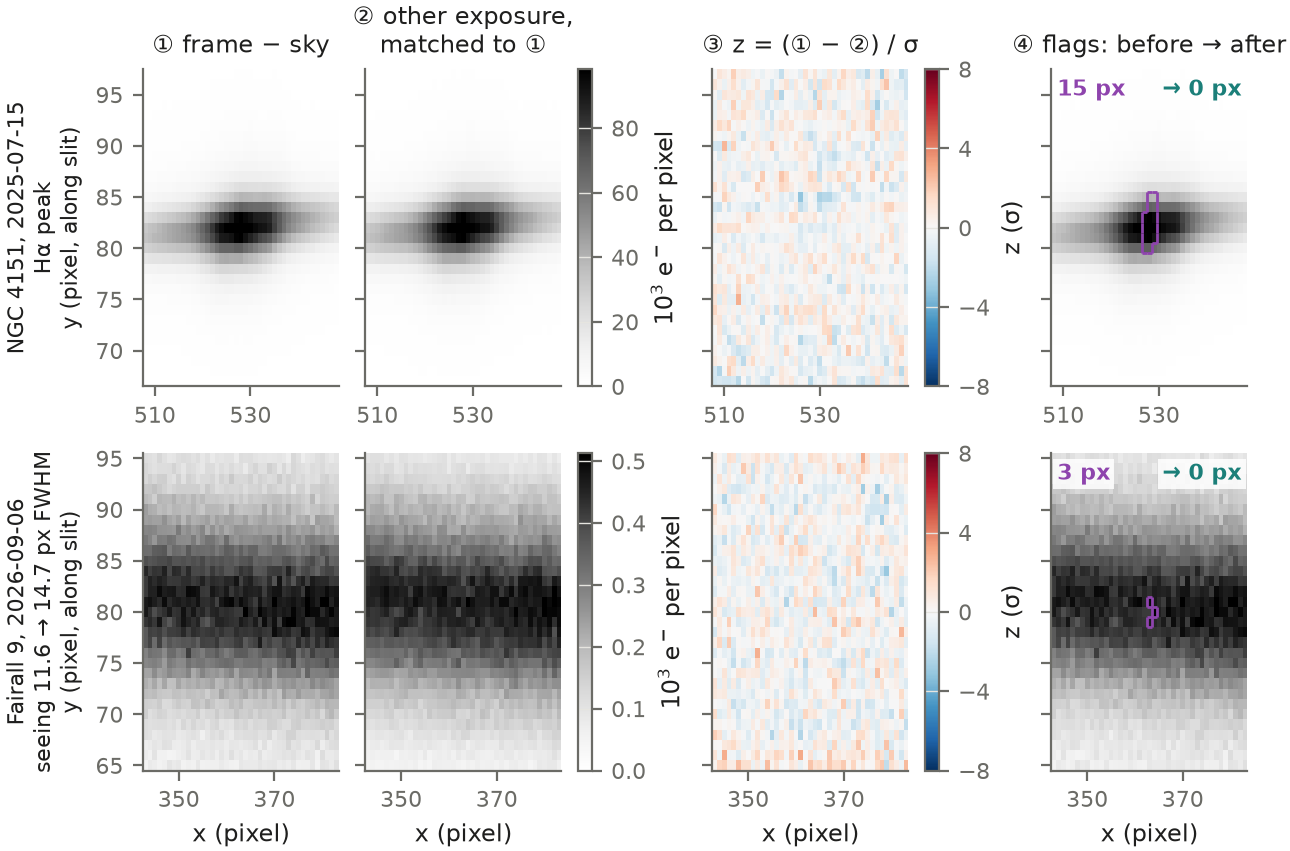
\includegraphics[width=\textwidth]{figures/fig_cr_pair.png}
\caption{The same-visit check on real pairs, both exposures reduced exactly as the stage sees them. Columns:
\ding{172} the frame minus its sky; \ding{173} the partner minus its sky, shifted onto the trace of the frame, scaled
per column, shifted along the dispersion and matched to the frame by the kernel along the slit (same grey scale as
\ding{172}); \ding{174} $z=($\ding{172}$-$\ding{173}$)/\sigma$, which is noise only where the two exposures show the
same thing; \ding{175} the flags of LA Cosmic with the object model (purple, before the check) and those left after the
check (teal; none here), with the number of flagged pixels in the panel. Rows: the H$\alpha$ peak of NGC\,4151 on 2025
July 15 (Figs.~\ref{fig:cr_halpha}, \ref{fig:cr_method}), 15 pixels removed; an LA Cosmic group on the trace of
Fairall\,9 that the partner shows to be real structure, in the visit where the FWHM changed from 11.6 to
14.7\,pixels, 3 pixels removed.}
\label{fig:cr_pair}
\end{figure}

% Results of the same-visit check (input from cr_pair.tex)
\subsection{Injection test with a partner}
\label{sec:cr_pair_inject}
We repeated the injection test of Section~\ref{sec:cr_inject} on eight frames that have a partner: four of NGC\,4151
at OGG and four of Fairall\,9 at COJ. In each frame we placed two random sets of 20 artificial cosmic rays in each of three
places: on the sky, on the trace, and on the line peaks or core. As real cosmic rays
are, they were injected into one exposure of the visit only. Each frame was then reduced three ways: with the 1.1.0
detector, with LA Cosmic and the object model, and with the object model followed by the same-visit check
(Table~\ref{tab:cr_pair_inject}).

\begin{table}[!htbp]
\centering\small
\caption{Injection test on frames with a partner: fraction of injected hits found (any pixel flagged), all hits and
those above 10 times the noise of their pixel, and the cosmic-ray pixels flagged in the same four frames without
injection. 160 hits per category and site (153 on the OGG peaks).}
\label{tab:cr_pair_inject}
\begin{tabular}{llccccc}
\toprule
Site & Detector & Sky & Trace & Line peak & Line peak & Pixels flagged \\
 & & & & or core & or core, $>10\sigma$ & without injection \\
 & & \multicolumn{4}{c}{(fraction of the hits detected)} & (pixels, 4 frames) \\
\midrule
OGG & 1.1.0 / improved v3 & 0.89 & 0.59 & 0.14 & 0.27 & 1037\\
    & object model & 0.89 & 0.76 & 0.50 & 0.89 & 1020\\
    & object model + same visit & 0.89 & 0.76 & 0.50 & 0.89 & 799\\
\midrule
COJ & 1.1.0 / improved v3 & 0.90 & 0.94 & 0.68 & 0.94 & 1775\\
    & object model & 0.90 & 0.94 & 0.79 & 1.00 & 1816\\
    & object model + same visit & 0.90 & 0.94 & 0.78 & 1.00 & 1634\\
\bottomrule
\end{tabular}
\end{table}

\textit{Result.} With the strict rule for new groups, the check finds the same artificial cosmic rays as the object
model alone. Of the 953 hits, none is found only with the check, and 2 are found only without it; both are faint hits on
Fairall\,9 line peaks (3.7--5$\sigma$, 7--12 per cent of the line). On the OGG line peaks, 8 hits above 10$\sigma$ are
missed by both; they carry 4--38 per cent of the line under them. An earlier version of the check, with the loose rule
for new groups, found 14 more hits on the sky and 6 more on the line peaks. But the same rule added hundreds of false
pixels on the narrow lines of the real sample (Section~\ref{sec:cr_pair}, item (iv)), and we chose clean lines.

What the check does is remove flags. In the frames without artificial cosmic rays it flags 22 per cent fewer pixels at
OGG and 10 per cent fewer at COJ. Per frame, it removes 9--19 LA Cosmic groups that the partner shows to be real
structure and adds 0--1; 35--51 groups per frame stay flagged because the partner cannot check them.

These runs were made before the rule for pixels flagged in both exposures on the object was added. That rule acts only
where the partner flagged the same pixel, and an artificial cosmic ray is in one exposure only, so the rule does not
change which of them are found.

% Same-visit check on the whole sample (input from cr_pair_results.tex)
\subsection{The whole sample}
\label{sec:cr_pair_sample}
We reduced all 106 exposures of the sample again with the check (60 of NGC\,4151 at OGG, 46 of Fairall\,9 at COJ).
Every one found its partner (\texttt{L1CRMETH} = \texttt{pair}). These products were made with the version of the
check \textit{before} the rule for pixels flagged in both exposures on the object (Section~\ref{sec:cr_pair}, step 8).
That rule was added after this run and measured on the seven frames with the most flags left on the lines; the sample
was not reduced again. Below, we call the version run on the sample the \textit{sample version}, and each number says
which version it comes from.

\paragraph{Flags on the narrow lines.} Table~\ref{tab:cr_pair_lines} counts the flagged pixels within 12\,\AA\ of
[O\,\textsc{iii}]\,$\lambda\lambda$4959,\,5007, H$\beta$ and H$\alpha$+[N\,\textsc{ii}] and within 8\,pixels of the
trace. On the NGC\,4151 lines, the first version of the check doubled the flags of the object model. The sample
version brings them to 215, fewer than with the object model alone (398) and with 1.1.0 (236), and it clears most of
the H$\alpha$ flags of 1.1.0. Fairall\,9 has few flags on its lines with any detector.

Most of these 215 pixels are still not cosmic rays. They are 0.32 per cent of the pixels in the line windows, against
0.003 per cent in five continuum windows on the same traces. Often both exposures of a visit are flagged at the same
line, which a cosmic ray cannot do. We found two causes in the worst frames. First, in good-seeing visits LA Cosmic
flags the same line and trace peaks in both exposures, so neither can check the other (item (v) of
Section~\ref{sec:cr_pair}). Second, on tilted lines a residual offset between the exposures leaves a
positive--negative pattern, whose positive half passes as a confirmed cosmic ray. The rule for pixels flagged in both
exposures removes the first cause (Table~\ref{tab:cr_pair_worst}). We left the second, because a rule for it would be
one more cut tuned on the frames it is meant to fix.

\begin{table}[!htbp]
\centering\small
\caption{Pixels flagged as cosmic rays on the narrow lines of the sample (within 12\,\AA\ of the line and 8\,pixels of
the trace), by order (1 red, 2 blue), for the 1.1.0 detector (improved v3 products), LA Cosmic with the object model, the
first version of the same-visit check, and the version run on the sample (before the rule for pixels flagged in both
exposures). Last rows: total, and frames with any flagged pixel.}
\label{tab:cr_pair_lines}
\begin{tabular}{llcccc}
\toprule
Target & Line, order & 1.1.0 & Object model & Check, first & Check, sample \\
 & & \multicolumn{4}{c}{(pixels)} \\
\midrule
NGC\,4151 & H$\alpha$+[N\,\textsc{ii}], 1 & 211 & 70 & 55 & 20 \\
(60 frames) & H$\beta$, 1 & 1 & 56 & 117 & 28 \\
 & H$\beta$, 2 & 0 & 6 & 0 & 0 \\
 & [O\,\textsc{iii}]\,4959, 1 & 0 & 42 & 71 & 31 \\
 & [O\,\textsc{iii}]\,4959, 2 & 24 & 74 & 139 & 45 \\
 & [O\,\textsc{iii}]\,5007, 1 & 0 & 89 & 170 & 77 \\
 & [O\,\textsc{iii}]\,5007, 2 & 0 & 61 & 288 & 14 \\
 & total & 236 & 398 & 840 & 215 \\
 & frames with any & 18 & 37 & 41 & 28 \\
\midrule
Fairall\,9 & total & 12 & 29 & 21 & 15 \\
(46 frames) & frames with any & 2 & 6 & 4 & 4 \\
\bottomrule
\end{tabular}
\end{table}

\begin{table}[!htbp]
\centering\small
\caption{The rule for pixels flagged in both exposures on the seven NGC\,4151 frames with the most flags on the
lines: pixels on the lines (as in Table~\ref{tab:cr_pair_lines}) flagged by LA Cosmic with the object model, by the
version run on the sample, and with the rule; and the LA Cosmic groups kept because the partner cannot check them
(mostly warm pixels, which the rule must not touch).}
\label{tab:cr_pair_worst}
\begin{tabular}{lccccc}
\toprule
Frame & \multicolumn{3}{c}{Pixels on the lines} & \multicolumn{2}{c}{Groups the partner cannot check} \\
 & LA + object model & sample version & with the rule & sample version & with the rule \\
\midrule
2025-03-27 0021 & 32 & 33 & 20 & 56 & 47 \\
2025-03-27 0020 & 24 & 19 & 13 & 56 & 48 \\
2025-05-31 0020 & 18 & 15 & 12 & 35 & 32 \\
2025-06-10 0006 & 21 & 26 & 22 & 6 & 5 \\
2025-06-10 0007 & 18 & 16 & 16 & 5 & 5 \\
2025-07-05 0004 & 17 & 14 & 14 & 23 & 23 \\
2025-07-14 0002 & 23 & 0 & 0 & 34 & 30 \\
\bottomrule
\end{tabular}
\end{table}

The rule is restricted to the object for a reason. When we applied it everywhere, it took the groups the partner
cannot check from 56 to 0 in the first frame of Table~\ref{tab:cr_pair_worst}. Cutouts showed that the extra groups it
removed off the trace were single warm pixels present in both exposures. On the object, the rule removes only line and
trace peaks, but it will also unflag a warm pixel that happens to lie on the trace. From the density of warm pixels
flagged in both exposures on the sky, we expect 4--7 such groups per frame. Each adds 50--90\,e$^-$ (at most
340\,e$^-$) to a column of the trace, which holds 30\,000--70\,000\,e$^-$ (6000\,e$^-$ in its faintest tenth): typically 0.1--0.3 per
cent of one of the 1700 columns, and at most $\approx6$ per cent (340\,e$^-$ in a column of 6000\,e$^-$). A map of the warm pixels, made from the flags that recur at the same place on the
detector in many frames, would remove them properly; we leave it for later.

\paragraph{The header keywords.} The keywords of the check give, per frame (median, with the range in brackets):
\begin{itemize}
\item \textit{OGG}: LA Cosmic flags 242 (115--715) pixels, of which 188 (96--681) remain after the check (80 per cent,
summed over all frames). 9 groups are confirmed, 12 removed, 34 kept because the partner cannot check them, and 0 (at
most 6) added. The partner cannot judge 0.1 per cent of the orders (at most 6 per cent). The offset along the
dispersion is at most 0.6\,pixel.
\item \textit{COJ}: 321 (175--1755) pixels flagged by LA Cosmic become 278 (129--1519), 90 per cent. 14 groups are
confirmed, 11 removed, 47 kept and 1 (at most 3) added. The partner cannot judge 0.2 per cent of the orders (at most
2.5 per cent).
\end{itemize}

\paragraph{Two faults found on the sample, and fixed.} The sample numbers in this section were measured before these
fixes.
\begin{enumerate}
\item[(i)] \textit{Spurious offsets along the dispersion.} In the blue order of six Fairall\,9 frames, the offset of
the partner along the dispersion came out at 1.4--3.4\,pixels, with the same sign for both exposures of a visit (2026
October 26: $-2.05$ and $-2.05$\,pixels; September 30: $-3.37$ and $-1.52$). A real offset cannot do this: if $b$ is
shifted with respect to $a$, then $a$ is shifted by the opposite amount with respect to $b$. The faint blue spectrum of
Fairall\,9 has no features above the noise. There the normalised cross-correlation peaks at only 0.09--0.26, against
0.92--1.00 in its red order and in both orders of NGC\,4151, and its peak lands wherever the noise puts it: leaving the
flagged cosmic-ray pixels out of the correlation moved one offset from $-2.05$ to $+2.22$\,pixels. An offset is now
used only where the peak exceeds 0.5, which separates the two groups cleanly.
\item[(ii)] \textit{New groups at the end of an order.} In the same frames the check added groups of 1--9 pixels right
at the end of the blue order (1\,pixel from it). There the signal stops sharply, and the matched partner misses the
step by a pixel. The 6-pixel margin in which no new group is added covered the edges of the orders along the slit, but
not their ends along the dispersion. It now covers the ends too.
\end{enumerate}
Measured again on the affected frames, the spurious offsets are gone (the red order keeps its offsets of
0.05--0.24\,pixel), and no group is added at an order end. The flags on the lines of the NGC\,4151 frames of
Table~\ref{tab:cr_pair_worst} are unchanged. Both faults have their own unit test (16 in all).

\paragraph{Fluxes.} What matters in the end is the flux. Table~\ref{tab:cr_pair_flux} gives the robust scatter of the
flux ratio of the two exposures of each visit, for the narrow lines and two continuum windows. This scatter is set by
the slit losses and the seeing, and the choice of detector changes it by 0.5 per cent or less. The one larger change,
for the red-order [O\,\textsc{iii}] of NGC\,4151 with the object model alone (2.5 against 1.7 per cent), is mostly
undone by the check (2.0 per cent). The optimal extraction rebuilds a masked pixel from the profile, so a false flag on
a line peak costs little flux, while a missed cosmic ray costs more. The gain that matters for the light curves is
therefore that of the object model: of the hits above 10$\sigma$ on the OGG line peaks, it finds 89 per cent, where
1.1.0 found 27 per cent (Table~\ref{tab:cr_pair_inject}). The same-visit check is a clean-up on top: 10--22 per cent
fewer flagged pixels (22 at OGG, 10 at COJ), a clean H$\alpha$ peak, and a mask that can be trusted on the lines.

\begin{table}[!htbp]
\centering\small
\caption{Robust scatter of the flux ratio of the two exposures of each visit (30 visits of NGC\,4151 at OGG, 23 of
Fairall\,9 at COJ), for the 1.1.0 detector (improved v3 products), LA Cosmic with the object model, and the same-visit check
(version run on the sample). [O\,\textsc{iii}]\,5007 from a doublet fit in each order; H$\alpha$+[N\,\textsc{ii}] for
NGC\,4151 only.}
\label{tab:cr_pair_flux}
\begin{tabular}{llccc}
\toprule
Target & Measurement & 1.1.0 & Object model & Same-visit check \\
 & & \multicolumn{3}{c}{(scatter of the ratio, per cent)} \\
\midrule
NGC\,4151 & [O\,\textsc{iii}]\,5007, blue order & 2.0 & 1.9 & 2.0 \\
 & [O\,\textsc{iii}]\,5007, red order & 1.7 & 2.5 & 2.0 \\
 & H$\alpha$+[N\,\textsc{ii}] & 2.5 & 2.3 & 2.5 \\
 & continuum, blue & 1.5 & 1.6 & 1.5 \\
 & continuum, red & 1.5 & 1.6 & 1.5 \\
\midrule
Fairall\,9 & [O\,\textsc{iii}]\,5007, blue order & 6.7 & 6.8 & 6.4 \\
 & [O\,\textsc{iii}]\,5007, red order & 6.7 & 6.6 & 6.8 \\
 & continuum, blue & 3.3 & 3.6 & 3.6 \\
 & continuum, red & 3.0 & 2.8 & 2.8 \\
\bottomrule
\end{tabular}
\end{table}


